\section{Khái niệm cơ bản}
\begin{frame}{Ví dụ đồ thị}
\centering
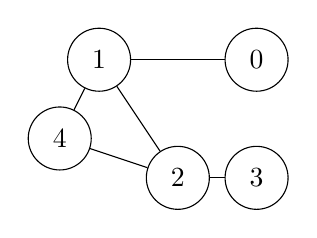
\begin{tikzpicture}[every node/.style={circle,draw,minimum size=8mm}]
\node (1) at (0,1) {1};
\node (2) at (1,-0.5) {2};
\node (3) at (2,-0.5) {3};
\node (4) at (-0.5,0) {4};
\node (0) at (2,1) {0};
\draw (1)--(4); \draw (1)--(0); \draw (1)--(2); \draw (2)--(3); \draw (4)--(2);
\end{tikzpicture}
\end{frame}